\section{Application existante}

\subsection{Présentation de l'application}
L'application sur laquelle nous travaillons est écrite en C++ avec l'utilisation de QtCreator. 
La bibliothèque de vision OpenCV  est largement utilisée dans le projet, le programme 
compile avec la version 2.4.8 d'OpenCV. Ce programme a été développé par les membres de l'équipe 
Fox. Cette application a fait l'objet de divers améliorations auparavant.\\

\subsection{Architecture}
L'application fournis est orientée objet et respect le principe <<open-close>>. En effet, celle-ci est 
découpé en Business Objects\footnote{Les Business Objects sont des objets métier qui s'occuppent de tâches 
précises}, il est possible de créer et greffer nos propres objets métiers dans l'application. Les Business 
Objects sont hiérarchisé dans une pyramide métier, où les objets métiers en haut de cette pyramide 
sont les plus abstrés et utilise les resultats de l'étages inférieur. Les objets métiers en bas de 
la pyramide sont les plus proche du flux vidéo brut.\\

\begin{figure}[H]
  \centering
  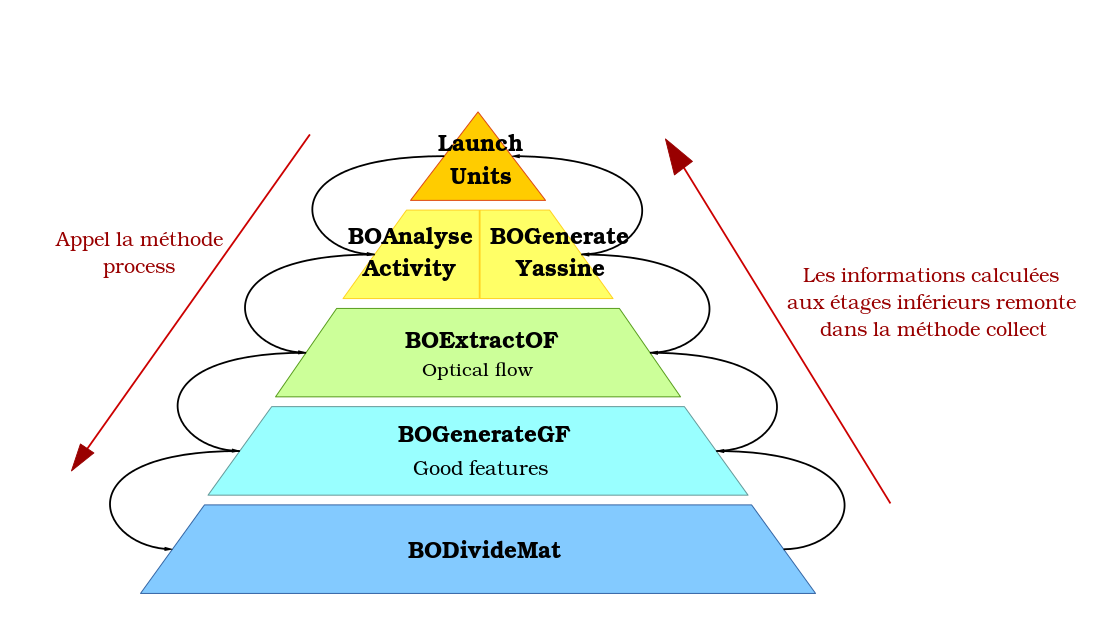
\includegraphics[width=12.5cm]{image/pyramide.png}
  \caption{Processus d'extraction des informations pyramidal sur le flux vidéo}
\end{figure}

Les différentes couches de la pyramide disposent d'une classe métier abstraite. Ces classes 
sont décrite dans la liste suivante :\\

\begin{itemize}
 \item \textbf{BODivideMat} : ces objets métiers découpent une image source plusieurs images tel que 
 le cadre du visage ou des yeux.
 \item \textbf{BOGenerateGF} : ces objets métiers générent les bonnes particularités (Good Features). 
 À cette étape, le choix des points d'intérêts est effectué, ces points sont dans la zone du visage 
 découpée dans l'étage précédente. Ensuite, les points identique dans l'image précédente et l'image 
 courrante sont conservés.
 \item \textbf{BOExtractOF} : ces objets métiers extraient les flux optiques (Optical Flows) à partir 
 des points générés lors de l'étape précédente. Les flux optiques représentent les mouvements à l'intérieur 
 du visage et doivent être invariants aux mouvement du visage, de la personne ou de la caméra.
 \item \textbf{BOAnalyseActivity et BOGeneteYassine} : ces objets métiers analysent les résultats 
 des flux optiques afin de déterminer les informations sur l'activité à l'intérieur du visage.
 \item \textbf{Lauch Units} : cette unitée n'est pas un objet métier, elle crée les objets métiers des 
 couches infèrieurs afin d'avoir une exécution du programme qui utilise ces Business Objects.
\end{itemize}
\ \\

Pour notre projet, nous travaillons dans la couche basse de la pyramide. Cette couche divise
les images du flux vidéo en diverses régions d'intérêt telles que la région du visage, puis 
des yeux.

\subsection{Reconnaissance du visage : Viola et Jones}
L'application est divisée en deux parties. La première recherche le visage grâce à
l'algorithme de Viola et Jones et la seconde recherche les yeux dans la région délimitée
précédemment.\\

L'algorithme de Viola et Jones\cite{Viola04robustreal-time} est une méthode qui a été créée pour la reconnaissance de visage dans une 
image. Cette méthode s'est par la suite généralisée à toutes sortes d'objets. L'algorithme nécessite une 
base de connaissances composée des caractèristiques de l'objet recherché. Cette base de connaissances est utilisé dans un 
apprentissage supervisé, c'est à dire que l'algorithme a besoin de données représentant
l'objet à détecter pour classifier les caractèristiques de celui-ci.\\

Cette algorithme est basé sur des caractèristiques pseudo-Haar qui crée des masques rectangulaires et adjacentes
dans différente zone de l'image. Chaque masque calcule l'intensité des pixels qu'il contient, puis l'algorithme fait
la différence entre les masque blanc et les masque noir. Cette méthode va permettre de détecter des contours ou des changements de 
texture.\\

\begin{figure}[H]
\center

\includegraphics[width=5cm]{image/pseudo_haar.png}
\caption{Exemple de caractèristiques pseudo-Haar utilisé pour l'algorithme Viola et Jones}
\end{figure}

Pour améliorer les perfomance de leur algorithme, Viola et Jones utilise la méthode Adaboost. Son
principe est de séléctionner les caractèristiques les plus performante pour la détection de l'objet grâce à
un calcule de probabilité utilisant l'entropie\footnote{valeur mesurant l'incertitude d'une données} des données.

\subsection{Détection des yeux}
Une fois que la région du visage est reconnue dans le flux vidéo, nous cherchons à détecter les yeux. 
L'algorithme de détection des yeux déjà existant dans l'application permet une détection des yeux 
robuste, mais accès peu précise. Cette algorithme consiste à scanner la région retrouver par la 
méthode de Viola et Jones et essayer de retrouver les yeux via une méthode Means Shift\footnote{technique 
d'analyse permettant de trouver les maxima dans une fonction de densité}



